\chapter{Stellar Structure and Evolution}
With the advent of spectroscopy and more formalized and globalized astronomy
during the 18th and 19th centuries a physically driven picture of stars emerged.
Spectroscopy revealed similar trends between our sun and other stars and new
physics and chemistry allowed astronomers to, in the early part of the 20th century, start piecing together that stars
were made, primarily, of extremely hot hydrogen and helium \citep{Payne1925}.

\begin{sidebar}{Kelvin-Helmholtz Lifespan}{gravCollapse}
  The total binding energy of a star may be approximated as
  \begin{equation*}
    U = -\frac{3}{5}\frac{GM^{2}}{R} \approx -2.3 \times 10^{41} \text{J}
  \end{equation*}
  The Sun's luminosity is approximatly $4\times 10^{26}$ J s$^{-1}$. Then
  assuming all of that energy is being produced by gravitational collapse the
  total time the sun could burn would be given by the ratio of the total energy
  to the luminosity.
  \begin{equation*}
    t = \frac{|U|}{L} \approx 19 \times 10^{6} \text{yr}
  \end{equation*}
\end{sidebar}

By the early 20th century astronomers were close to figuring out what energy
powered stars. The most prominent theory being heat generated from
gravitational collapse \citep[which had initially been proposed as a theory of
stellar system, but not energy generation by Kant and Laplace,][]{Kalita2023}.
Lord Kelvin and Hermann von Helmholtz proposed that a stars energy could
originate from gravitational collapse. They derived that the sun could power
itself for 19 million years \addcite (Aside \ref{gravCollapse}). However, as
geological records settled on an age in the billions of years for earth it
became clear that some other mechanism must provide energy to a star.

Arthur Eddington, often considered one of the founders of stellar astrophysics,
concerned with discrepancy between geological records of Earths age and the
suns maximum life span, as predicted by the Kelvin-Helmholtz mechanism,
proposed in the 1920s that a stars energy might primarily originate from the
fusion of hydrogen into helium \addcite. Early estimates of the maximum
lifespan of the sun if it were powered by hydrogen fusion proved to be
sufficient for the Earths lifespan to make sense. In the following decades the
sun and other stars would become important test beds for physics too extreme to
be studied in laboratory conditions on earth, a theme similar to one we will
return to multiple times during this thesis.

While the mechanism which powers the sun was still being debated mathematical
models which would evolve into those still used today were being developed.
Over the last half of the 19th and first decade of the 20th centuries Lane,
Ritter, and Emden codified the earliest mathematical model of stellar
structure, a ball of gas whos perssure depends only on its density, (Equation
\ref{eqn:polytrope}), in \textit{Gaskugeln} (Gas Balls) \citep{Emden1907}.

\begin{align}\label{eqn:polytrope}
	\frac{d}{d\xi}\left(\xi^{2}\frac{d\theta}{d\xi}\right) = -\xi^{2}\theta^{n}
\end{align}

Where $\xi$ and $\theta$ are dimensionless parameterizations of radius and
temperature respectively, and $n$ is known as the polytropic index (Figure
\ref{fig:runofp}). Despite this early work, it wasn't until the late 1930s and
early 1940s that the full set of equations needed to describe the structure of
a steady state, radially-symmetric, star (known as the equations of stellar
structure) began to take shape as the specific fusion chains (primarily the
proton-proton chains and the Carbon-Nitrogen-Oxygen cycle) were, seriously
considered as energy generation mechanisms \citep{Cowling1966}. Since then, and
especially with the proliferation of computers in astronomy, the equations of
stellar structure have proven themselves an incredibly predictive set of
models.  

\begin{figure}[htbp]
  \centering
  \begin{subfigure}[t]{0.45\textwidth}
    \centering
    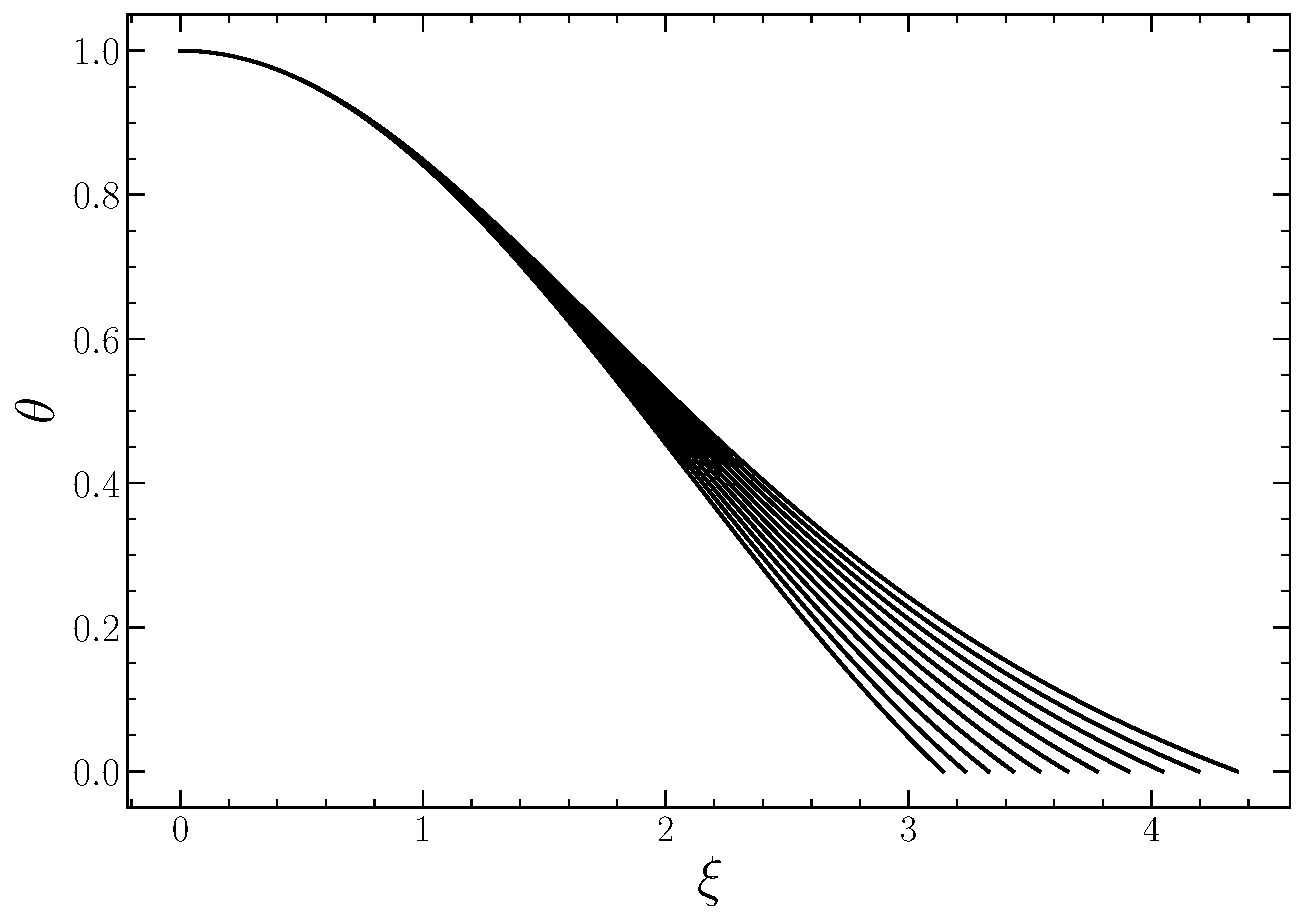
\includegraphics[width=\textwidth]{figures/introduction/runofp.pdf}
    \caption{Solutions to the lane-emden equation for a run of polytropic
    indexes. From left to right the solutions range from an index of 1 to 2
    with a step of 0.1.}
    \label{fig:runofp}
  \end{subfigure}
  \begin{subfigure}[t]{0.45\textwidth}
      \centering
      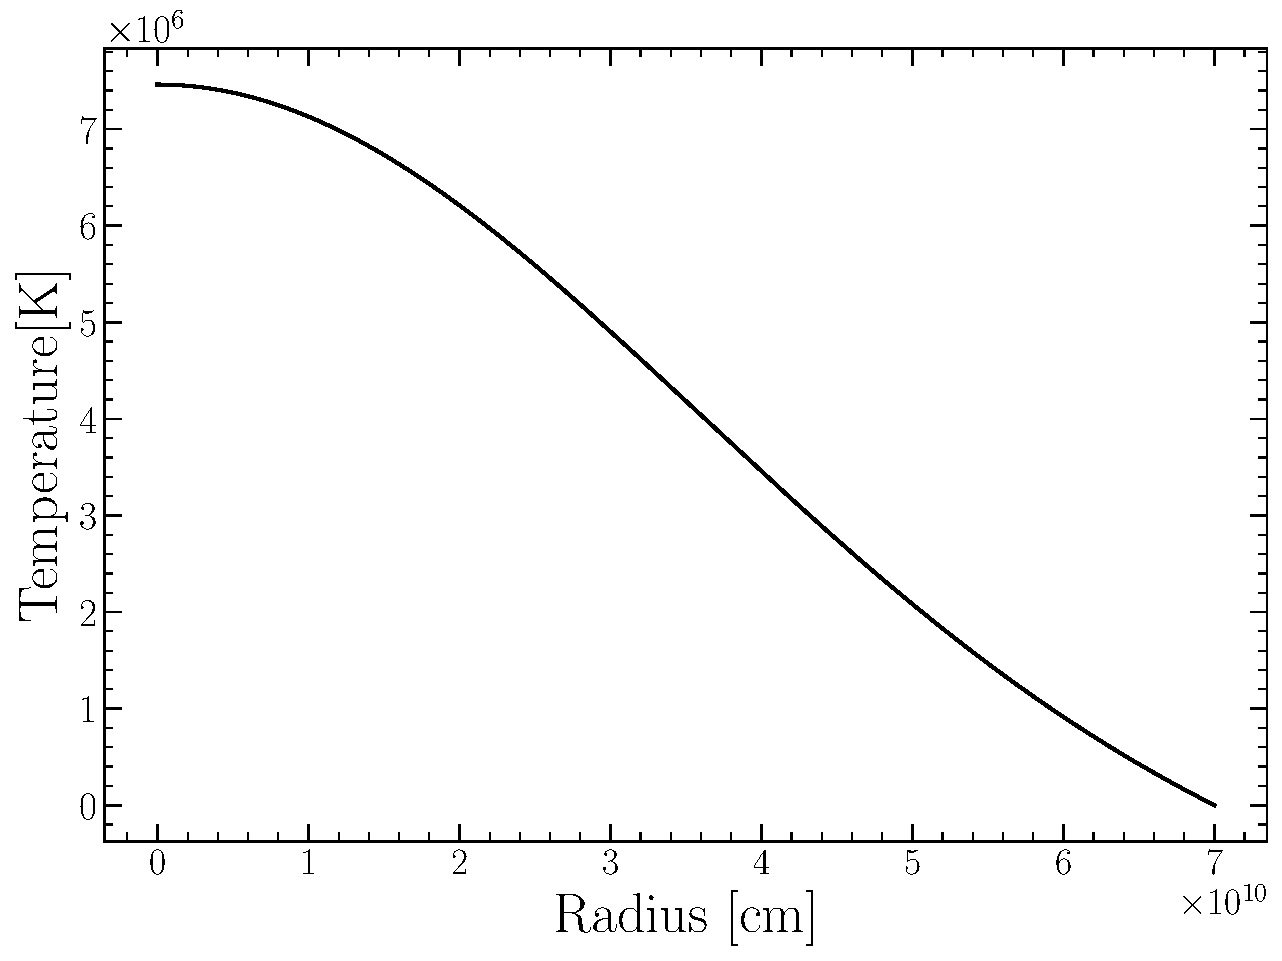
\includegraphics[width=\textwidth]{figures/introduction/PolytropeTempProfile15.pdf}
      \caption{Solution to the lane-emden equation for a polytropic index of 1.5 scaled to
      physical values for a star the mass and radius of our sun.}
      \label{fig:polyScaled}
  \end{subfigure}
  \caption{Various ways to visualize the solutions of a polytropic equation of state.}
  \label{fig:starsInHistory}
\end{figure}


Today stars and stellar physics form the basis of much of astronomy \addcite.
Despite being some of the smallest objects studied by astronomers stars provide
the majority of the luminosity of the universe \addcite. They make up key
rungs on the distance ladder \addcite, and they provide key constraints on
topics as varied as fundamental nuclear physics \addcite and the search for
habitable planets and life \addcite. Stars then represent not just an interesting
object of study in their own right but also, in the right conditions, labratories
where we can study astronomical objects in a controlled manner.

\section{Equations of Stellar Stucture}
Solutions to the Lane-Emden equation (Equation \ref{eqn:polytrope}) can be
scaled from $\xi$ and $\theta$ to physical quantities given some total mass and
radius (Figure \ref{fig:polyScaled}). However, these solutions are not, in and
of themselves, enough to describe the 1D structure of a star. From the
Lane-Emden equation mathematical models of stars have evolved into a series of
four coupled differential equaitons with are used to describe the structure of
radially symmetric stellar models, these are known as the equations of stellar
structure (Aside \ref{stellarStructEQN}). These equatiions, in addition to what
stellar structure theorists call ``microphysics'' and an equation of state
define the steady state structure of a one dimensional stellar model. To take a
steady state model such as this and evolve it over time stellar structure
programs alternate between updating the structure and updating nuclear reaction
rates based on this updated structure. This model of stars has prooven
incredibly predictive and has allowed for controlled studies of stars and
stellar populations, a key element of modern astrophysics.

\begin{sidebar}[l]{Equations of Stellar Stucture}{stellarStructEQN}

  \textbf{Hydrostatic Equilibrium}: $\frac{dP}{dr} = -\frac{Gm\rho}{r^{2}}$

  \textbf{Mass Continuity}: $\frac{dm}{dr} = 4\pi r^{2}\rho$

  \textbf{Luminosity}: $\frac{dl}{dr} = 4\pi r^{2}\rho(\epsilon - \epsilon_{\nu})$

  \textbf{Energy Transport (radiative)}: $\frac{dT}{dr} = -\frac{3\kappa\rho l}{64\pi r^{2}\sigma T^{3}}$
\end{sidebar}

There are currently many stellar structure codes \citep[e.g.][]{Dotter2008,
Kovetz2009, Paxton2011} which integrate the equations of stellar structure ---
in addition to equations of state and lattices of nuclear reaction rates ---
over time to track the evolution of an individual star. The Dartmouth Stellar
Evolution Program (DSEP) \citep{Chaboyer2001, Bjork2006, Dotter2008} is one
such, well tested, stellar evolution program.

DSEP solves the equations of stellar structure using the Henyey method
\citep{Henyey1964}. This is a relaxation technique making use of a
Newton–Raphson root finder and therefore requires some initial guess to relax
towards a solution. This guess will be either some initial, polytropic, model
or the solution from the previous timestep.  In order to evolve a model through
time DSEP alternates between solving for reaction rates and the structure
equations. At some temperature and pressure from the solution to the structure
equations DSEP finds the energy generation rate due to proton-proton chains,
the CNO cycle, and the tripe-alpha process from known nuclear cross sections.
These reaction rates yield both photon and neutrino luminosities as well as
chemical changes over some small time step. Thermodynamic variables are
calculated using an equation of state routine which is dependent on the initial
model mass. All the updated physical quantities (pressure, luminosity, mean
molecular mass, temperature) are then used to solve the structure equations
again. This process of using a solution to the structure equations to calculate
reaction rates which then inform the next structure solution continues until
DSEP can no longer find a solution.  This can happen as the stellar structure
equations are extremely stiff. In addition, for finite radial mesh sizes,
discontinuities can occur.

While other stellar evolution programs, such as the widely used Modules for
Experimentation in Stellar Astrophysics (MESA) \citep{Paxton2011}, consider a
more complex handling of nuclear reaction rate calculations, and are
consequently more applicable to a wider range of spectral classes than DSEP,
DSEP has certain advantages over these other programs that make it well suited
for certain tasks, such as low-mass modeling. For one, DSEP generally can
evolve models much more rapidly than MESA and has a smaller memory footprint
while doing it. This execution time difference is largely due to the fact that
DSEP makes some simplifying assumptions due to its focus only on models with
initial masses between 0.1 and 5 M$_{\odot}$ compared to MESA’s more general
approach.  Moreover, MESA elects to take a very careful handling of numeric
uncertainty, going so far as to guarantee byte-to-byte similarity of the same
model run on different architectures \citep{Paxton2011}. DSEP on the other hand
makes no such guarantee. Rather, models evolved using DSEP will be accurate
down to some arbitrary, user controllable, tolerance but beyond that point may
vary from one computer to another. Despite this trade off in generality and
precision, the current grid of isochrones generated by DSEP \citep{Dotter2008},
has been heavily cited since its initial release in 2008, proving that there is
a place for a code as specific as DSEP.
